\documentclass[a4paper]{article}

\usepackage[english]{babel}
\usepackage{graphicx}           % For including graphics.
\usepackage{amsmath}            % Some mathematical symbols.
\usepackage{hyperref}           % To use some cool links within the report.
	\hypersetup{colorlinks=true}
\usepackage[center]{caption}    % The name should be enough description :D
\usepackage[numbered, framed, useliterate]{mcode}

\addtolength{\topmargin}{-20mm}% Margin adjustments.
\addtolength{\textheight}{20mm}% Margin adjustments.

\begin{document}

\title{EN2202 Pattern Recognition\\
Assignment 1 - HMM Signal Source}
\author{Fernando J. Iglesias Garc\'{i}a \\ fjig@kth.se
	\and
	Bernard Hern\'{a}ndez P\'{e}rez \\ bahp@kth.se }

\maketitle

\begin{itemize}
\item Consider the following infinite duration HMM $\lambda$ = \{q, A, B\}

\begin{equation}
	\label{eq:def_hmm1}
	q = \begin{pmatrix} 0.75 \\ 0.25 \end{pmatrix};
	A = \begin{pmatrix} 0.99 & 0.01 \\ 0.03 & 0.97 \end{pmatrix}
	B = \begin{pmatrix} b_1(x) \\ b_2(x) \end{pmatrix}
\end{equation}

\noindent
where $b_1(x)$ is a scalar Gaussian density function with mean
$\mu_1=0$ and standard deviation $\sigma_1=1$, and $b_2(x)$ is a similar
distribution with mean $\mu_2=3$ and standard deviation $\sigma_2=2$.

\begin{itemize}

	\item \emph{What are the values of $P(S_t=j)$, $j \in \{1,2\}$ for
		$t = 1,2,3...$ \linebreak theoretically calculated and the corresponding
		measured values?}

	The initial state probability distribution defines entirely $P(S_1=j)$,
	this is
	~
	\begin{equation*}
		\mathbf{P}_1 = q = \begin{pmatrix} P(S_1=1) \\ P(S_1=2) \end{pmatrix} =
				\begin{pmatrix} 0.75 \\ 0.25 \end{pmatrix}
	\end{equation*}

	To obtain the probability distribution in the next state,
	~
	\begin{equation}
		\label{eq:next_dist}
		\mathbf{P}_t = A^T \cdot \mathbf{P}_{t-1}
	\end{equation}

	Using the values of this particular problem it is obtained that
	~
	\begin{equation*}
		\mathbf{P}_2 = 
		\begin{pmatrix} 0.99 & 0.03 \\ 0.01 & 0.97 \end{pmatrix} \cdot
		\begin{pmatrix} 0.75 \\ 0.25 \end{pmatrix} = 
		\begin{pmatrix} 0.75 \\ 0.25 \end{pmatrix}
	\end{equation*}

	This probability distribution is still equal to $q$, the probability
	of being in state 1 at timestep $t=2$ is three times larger than
	being in state 2. This, together with the fact that the elements of
	$A$ remain constant for all $t$, implies that the computations of
	$P(S_t=j)$, $j \in \{1,2\}$ for $t>1$ are identical to the ones shown
	above. Therefore, $P(S_t)$ is constant for all $t$ or, in other words,
	the HMM is \emph{stationary}.

        \vspace{2mm}
	Using Markov chain's \texttt{rand} function to generate a sequence of
	length $T=10~000$, the relative frequencies obtained
	experimentally of \linebreak occurrence of states $S_t=1$ and $S_t=2$ are:

	\begin{center}
		\begin{tabular}{ | c | c | }
			\hline
			$\hat{P}(S_t=1)$ & $\hat{P}(S_t=2)$ \\
			\hline
			0.7341 & 0.2659 \\
			\hline
		\end{tabular}
	\end{center}

	\item \emph{What are the values of ${\rm E}[X_t]$ and ${\rm Var}[X_t]$
		theoretically calculated and the corresponding measured values?}
	~
	\begin{align*}
            {\rm E}[X_t] = {\rm E}_{S_t}[X_t|S_t] =& {\rm E}[X_t|S_t=1] \cdot P(S_t=1) + \\  
                                                   &{\rm E}[X_t|S_t=2] \cdot P(S_t=2) = \\
                                                  =& 0 \cdot 0.75 + 3 \cdot 0.25 = \framebox{0.75}
	\end{align*}

	\begin{align*}
		{\rm Var}[X_t] = {\rm E}_{S_t}[ {\rm Var}_{X_t}[X_t|S_t] ] + 
			{\rm Var}_{S_t}[{\rm E}_{X_t}[X_t|S_t]]
	\end{align*}

	\begin{align*}
            {\rm E}_{S_t}[ {\rm Var}_{X_t}[X_t|S_t] ] =&
			{\rm Var}[X_t|S_t=1] \cdot P(S_t=1) + \\
                       &{\rm Var}[X_t|S_t=2] \cdot P(S_t=2) = \\
                        =& 1 \cdot 0.75 + 4 \cdot 0.25 = \underline{1.75}
	\end{align*}			
	\begin{align*}
		{\rm Var}_{S_t}[{\rm E}_{X_t}[X_t|S_t]] &=
		{\rm E}_{S_t}[ ( {\rm E}_{S_t}[X_t|S_t] - {\rm E}_{S_t}[{\rm E}_{S_t}[X_t|S_t]])^2 ] \\
		&= 0.75 \cdot [ (0-0.75)^2 ] + 0.25 \cdot [ (3-0.75)^2 ] = \underline{1.6875}
	\end{align*}
	\begin{align*}
		{\rm Var}[X_t] = {\rm E}_{S_t}[ {\rm Var}_{X_t}[X_t|S_t] ] + 
		{\rm Var}_{S_t}[{\rm E}_{X_t}[X_t|S_t]] = \framebox{3.4375}
	\end{align*}

	Finally, using HMM's \texttt{rand} function to generate a sequence of
	$T = 10~000$ output scalar random numbers, the mean and variance
	computed in MATLAB are


	\begin{center}
		\begin{tabular}{ | c | c | }
			\hline
			$\hat{{\rm E}}[X_t]$ & $\hat{{\rm Var}}[X_t]$ \\
			\hline
			0.7871 & 3.5510 \\
			\hline
		\end{tabular}
	\end{center}

	\item Figure~\ref{fig:output_hmm1} shows 500 contiguous observations
	generated by the HMM. The output of this HMM is characterized by two
	levels, one centered around 0 and the other around 3. These levels
	correspond to the states of the HMM. Also, it can be seen that the
	observations fluctuate considerably. This is one of the random
	components of the HMM and it stems from the definition of the
	observations as Gaussian density functions. Note too that the
	fluctuation in the lower level is smoother than the one in the higher
	level. This derives from the fact that the state characterized with a
        zero mean Gaussian has smaller standard deviation than the other state.

	\begin{figure}[!ht]
	\centering
	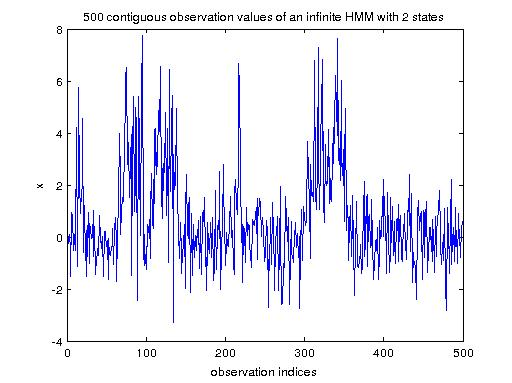
\includegraphics[width=0.85\columnwidth]{figures/1_1.jpg}
	\caption{500 contiguous output samples taken from the HMM defined in
	Equation~\eqref{eq:def_hmm1}.}
	\label{fig:output_hmm1}
	\end{figure}

\end{itemize}

\item Now a new HMM is created, identical to the one defined in
Equation~\eqref{eq:def_hmm1} but with both means equal to zero for the
observation distributions of both states, i.e. $\mu_1 = \mu_2 = 0$.
Figure~\ref{fig:output_hmm2} shows 500 observations generated by this new HMM.
Comparing this plot with the one produced by the former HMM shown in
Figure~\ref{fig:output_hmm1}, in both of them two different patterns are
observed. In other words, both HMMs have in common their number of states, equal
to two. On the other hand, the output of the second HMM fluctuates around the
same level whereas there are clearly two different levels in the output of the
first HMM. This reflects the fact that the two states of the first HMM have
Gaussian output distributions with different mean values while the Gaussians of
the second HMM are both zero mean.

\vspace{2mm}
\noindent
Even though it may be probably more difficult to estimate the state sequence
$\underbar{S}$ of the underlying Markov chain of the second HMM from the
output $\underbar{x}$, it is still possible as long as the output
distributions of the states are not exactly the same. In this case, the standard
deviations are different.

\begin{figure}[!ht]
\centering
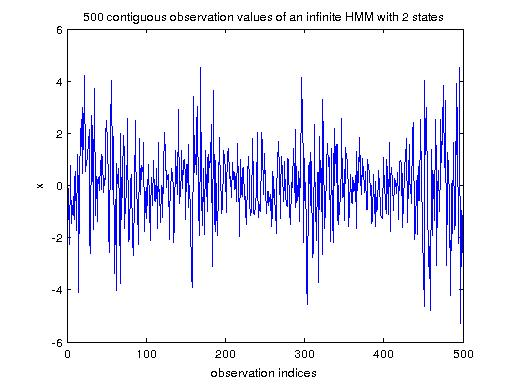
\includegraphics[width=0.85\columnwidth]{figures/1_2.jpg}
\caption{500 contiguous output samples taken from the HMM defined in
Equation~\eqref{eq:def_hmm1} modified so both output distributions have zero mean.}
\label{fig:output_hmm2}
\end{figure}

\item Consider the finite-duration Markov chain $\text{M} = \left\{q, A\right\}$
defined in~\eqref{eq:def_hmm2}, where the last column of A denotes the
probability to stop from every state of the chain.

\begin{equation}
	\label{eq:def_hmm2}
	q = \begin{pmatrix} 0.75 \\ 0.25 \end{pmatrix};
        A = \begin{pmatrix} 0.98 & 0.01 & \vline & 0.01 \\
                            0.02 & 0.97 & \vline & 0.01 \end{pmatrix}
\end{equation}

\noindent
Instead of defining a finite-duration HMM, only the Markov chain part has been
defined since in this exercise just the length of the output sequences are
of interest. 

\pagebreak

\vspace{2mm}
\noindent
The probability to stop defined in Equation~\eqref{eq:def_hmm2} is the same
for every state and equal to 0.01 or, in other words, on average one out of a
hundred transitions from any of the states the state sequence generated by the
Markov chain ends.

\vspace{2mm}
\noindent
The following piece of MATLAB code creates the Markov chain defined
in~\eqref{eq:def_hmm2}, generates N sequences of states and computes their
average length. Note that even if a large number is given to Markov chain's
\texttt{rand} function, the sequence generated is likely to be shorter than that
since this is a finite-duration Markov chain.

\lstinputlisting{scripts/s1_1.m}

\noindent
The output of one execution gives 105.76 as result for the average length,
value close to what was expected.

\item Finally, the code used to verify that vector-valued output distributions
work correctly is shown:

\lstinputlisting{scripts/s1_2.m}

\end{itemize}
\end{document}
